% Copyright 2004 by Till Tantau <tantau@users.sourceforge.net>.
%
% In principle, this file can be redistributed and/or modified under
% the terms of the GNU Public License, version 2.
%
% However, this file is supposed to be a template to be modified
% for your own needs. For this reason, if you use this file as a
% template and not specifically distribute it as part of a another
% package/program, I grant the extra permission to freely copy and
% modify this file as you see fit and even to delete this copyright
% notice. 
\documentclass[hyperref={pdfpagelabels=false}]{beamer}
\usepackage{tabu}
%\documentclass{beamer}
% Replace the \documentclass declaration above
% with the following two lines to typeset your 
% lecture notes as a handout:
%\documentclass{article}
%\usepackage{beamerarticle}
%\usepackage{xgreek}
%\usepackage[english,greek]{babel}
%\usepackage[utf8]{inputenc}
%\selectlanguage{english}
%\usepackage[T1]{fontenc}
%\sepackage{xgreek}
%\usepackage[Greek,Latin]{ucharclasses}
%\setTransitionsForGreek{\setlanguage{greek}}{\setlanguage{english}}
%\usepackage{fontspec}
%\setmainfont{Times New Roman} % substitute with any font that exists on your system
%\setsansfont{Times New Roman} % substitute with any font that exists on your system
%\setmonofont{Times New Roman} % substitute with any font that exists on your system
%\usepackage{ucs}
%\usepackage{verbatim}
%\usepackage{xltxtra}
%\usepackage{bm}
%\setmainfont{Times New Roman}
%\usepackage{polyglossia}
%\setmainlanguage[variant=mono]{greek}
%\setotherlanguage{english}
%\newfontfamily\greekfont{Times New Roman}
\usepackage{fontspec}
\usepackage[Latin,Greek]{ucharclasses}
\newfontfamily\greekfont{Times New Roman}[
Scale=MatchUppercase
]
\setTransitionsForGreek{\begingroup\greekfont}{\endgroup}
%\usepackage[greek,english]{babel}
%\usepackage[utf8x]{inputenc}
%\newcommand{\en}{\selectlanguage{english}}
%\newcommand{\el}{\selectlanguage{greek}}
% There are many different themes available for Beamer. A comprehensive
% list with examples is given here:
% http://deic.uab.es/~iblanes/beamer_gallery/index_by_theme.html
% You can uncomment the themes below if you would like to use a different
% one:
%\usetheme{AnnArbor}
%\usetheme{Antibes}
%\usetheme{Bergen}
%\usetheme{Berkeley}
%\usetheme{Berlin}
%\usetheme{Boadilla}
%\usetheme{boxes}
%\usetheme{CambridgeUS}
%\usetheme{Copenhagen}
%\usetheme{Darmstadt}
%\usetheme{default}
%\usetheme{Frankfurt}
%\usetheme{Goettingen}
%\usetheme{Hannover}
%\usetheme{Ilmenau}
%\usetheme{JuanLesPins}
%\usetheme{Luebeck}
%\usetheme{Madrid}
%\usetheme{Malmoe}
%\usetheme{Marburg}
%\usetheme{Montpellier}
%\usetheme{PaloAlto}
%\usetheme{Pittsburgh}
%\usetheme{Rochester}
%\usetheme{Singapore}
%\usetheme{Szeged}
\usetheme{Warsaw}
\usecolortheme{beaver}
\usepackage{tikz}
\usetikzlibrary{arrows}

\title{Lamda Calculus}
%\setbeamerfont{Times New Roman}{family=\rm}
% A subtitle is optional and this may be deleted
\subtitle{Optional Subtitle}

\author{Nikos Zarifis\inst{1}}
% - Give the names in the same order as the appear in the paper.
% - Use the \inst{?} command only if the authors have different
%   affiliation.

\institute[Universities of Somewhere and Elsewhere] % (optional, but mostly needed)
{
  \inst{1}%
  ECCE\\
  National Technical University of Athens}
% - Use the \inst command only if there are several affiliations.
% - Keep it simple, no one is interested in your street address.

\date{5  10, 2015}
% - Either use conference name or its abbreviation.
% - Not really informative to the audience, more for people (including
%   yourself) who are reading the slides online

\subject{Category Theory}
% This is only inserted into the PDF information catalog. Can be left
% out. 

% If you have a file called "university-logo-filename.xxx", where xxx
% is a graphic format that can be processed by latex or pdflatex,
% resp., then you can add a logo as follows:

% \pgfdeclareimage[height=0.5cm]{university-logo}{university-logo-filename}
% \logo{\pgfuseimage{university-logo}}

% Delete this, if you do not want the table of contents to pop up at
% the beginning of each subsection:
\AtBeginSubsection[]
{
  \begin{frame}<beamer>{Outline}
    \tableofcontents[currentsection,currentsubsection]
  \end{frame}
}

% Let's get started
	\begin{document}

\begin{frame}
  \titlepage
\end{frame}

\begin{frame}{Outline}
  \tableofcontents
  % You might wish to add the option [pausesections]
\end{frame}
 	
% Section and subsections will appear in the presentation overview
% and table of contents.
\section{Ορισμοί}

\subsection{Τι είναι κατηγορία;}

\begin{frame}
	\frametitle {Ορισμός Κατηγορίας}
  \begin{itemize}
  \item {

    Ένα σύνολο απο αντικείμενα. Συμβολίζουμε ως }:  obj(C).
  
  \item {

    Ένα σύνολο απο μορφισμούς. Πχ $f:A\rightarrow B $. Συμβολίζεται $hom_C(a,b)$.
  }
  \item {
		  Την πράξη σύνθεση. Όπως γίνεται η Σύνθεση συναρτήσεων.\\
		  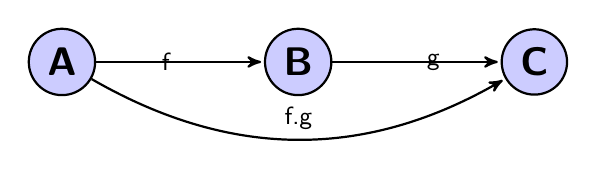
\begin{tikzpicture}[->,>=stealth',shorten >=1pt,auto,node distance=3cm,
  thick,main node/.style={circle,fill=blue!20,draw,font=\sffamily\Large\bfseries}]

  \node[main node] (1) {A};
  \node[main node] (2) [right of=1] {B};
  \node[main node] (3) [right of=2] {C};

  \path[every node/.style={font=\sffamily\small}]
    (1) edge node [left] {f} (2)
        edge [bend right] node {f.g} (3)
    (2) edge node [right] {g} (3);
\end{tikzpicture}
\\	Συμβολίζουμε την σύνθεση με την .(dot). 
	Κι έχουμε 2 αξιόματα:Προσετεριστική κι την ύπαρξη ουδέτερου στοιχίου.
	 }
  \end{itemize}
\end{frame}


\begin{frame}
	\frametitle{Functors}
Έστω ότι έχουμε 2 κατηγορίες, μπορούμε να όρισουμε μια συνάρτηση απο τα αντικείμενα της κατηγορίας Α στην Κατηγορία Β. 
\\ \begin{example} Έστω $F:C_A->C_B$,$a\in obj(A) \rightarrow F(a)\in obj(B)$\end{example}.Όπως επίσης αν έχω εναν μορφισμό  $f:a_A->b_A$  
\\ τότε $F(f): F(a_A)->F(b_A)$.\\ Για την σύνθεση ισχυεί: $F(f.g)=F(f).F(g)$\\ και ως προς το ουδέτερο μορφισμό $F(id_A)=id_{F(A)}$
%\includegraphics[width=100pt,height=100pt]{Functor.png}
\end{frame}

\begin{frame}
	\frametitle{Αρχικά - Τελικά Αντικείμενα}
Έχουμε επίσεις:
\begin{itemize}
\item
{
	\textbf {Intial Obj} : Αρχικό Αντικείμενο : Για κάθε άλλο αντικείμενο τις κατηγορίας υπάρχει ακριβώς ενας μορφισμός που να πηγαίνει σε αυτο.
\pause
}
\item{
		\textbf{Terminal obj} : Τελικό Αντικείμενο: Είναι το δυικό του αρχικού, δηλαδή 	για κάθε αντικείμενο υπάρχει ακριβώς ένανς μορφισμός που να πηγαίνει στο τελικό
}
\end{itemize}
\end{frame}

\begin{frame}
	\frametitle{Δυική κατηφορία}
Σε κάθε κατηγορία μπορούμε να όρισουμε μια κατηγορία όπου κάθε μορφισμός που υπάρχει στον κανόνικο , υπάρχει στο δυικό με αντιστρεμένα τα άκρα.
Το αρχικό αντικείμενο γίνεται τελικό κι αντίστροφα.
\\
Ισχυεί: $G=f.g \rightarrow G^{op}=g^{op}.f^{op}$ .
\\
\textbf {Παραδείγματα}
\begin{itemize}
\item
{
Αν πάρουμε ως αντικείμενα το $N$ κι όλους τους 1-1 μορφισμούς. Πχ : f(n)=n+1 . Δυικό το f(n)=n-1 .Αρχικό το 0, Τελικό δεν έχει.
\pause
}
\item<2->
{
Στους Δυανισμάτικους χώρους αν πάρουμε ως αντικείμενα όλα τα δυανίσματα, κι ως μορφισμούς όλους τους μορφισμούς τάξης n. Πχ Ο πίνακας Α κι ο δυικός που είναι ο $A^{-1}$.

}
\end{itemize}
\end{frame}
\begin{frame}
	\frametitle{Cartesian Closed Categories}
Έστω μια κατηγορια C λέμε ότι είναι Cartesian Closed (CCC) ανν:
\begin{itemize}
\item
{
Έχει τερματικό αντικείμενο.
\pause
}
\item <2->
{
Για κάθε 2 αντικείμενα στην C , έχουμε κι το X*Y στην C. 
}
\item <3->
{
Για κάθε 2 αντικείμενα στην C , έχουμε κι το $X^Y$ στην C. 
}
\end{itemize}

\end{frame}

\begin{frame}
	\textbf{	Products}:
Θα λέμε ότι ένα αντικείμενο είναι product (γινόμενο) 2 αντικείμενον ανν όριζουμε 2 μορφιφούς προβολών του Χ, έστω $X=X_1*X_2$
\\ \begin{itemize}
        \item {$\pi_1 : X\rightarrow X_1$ }
        \item <2-> {$\pi_2 : X\rightarrow X_12$}
\uncover <3->{\\
Και επίσεις έστω οι μορφισμοί $f: Y\rightarrow X$ και $f_1: Y\rightarrow X_1$ , $f_2: Y\rightarrow X_2$ έτσι ώστε: $f(Y)= f_1(Y)*f_2(Y)$.\\ Κι σε σχήμα:
\\ \includegraphics[height=80pt,width=80pt]{product.png}}
\end{itemize}

\end{frame}

\begin{frame}
	\textbf{Expomential Object}:
Αν έχουμε 2 αντικείμενα στην κατήγορία όριζουμε ως $X^Y$ το σύνολο των μορφισμων απο το Υ, Χ .
\\Κι θα ορίσουμε με την σείρα μας 2 πολύ συμαντικές συναρτήσεις:
Την eval $eval_{A,B}: B^A * A \rightarrow B$ .\\ Όπως φαίνεται κι απο τον τύπο
ισχυεί ότι $eval_{A,B}(f,A)=f(A)$.
\\ Και την curry έτσι ωστε αν έχουμε έναν μορφισμό g τότε $curry_c(g) : C\rightarrow B^A$ και ισχυεί οι $eval_{A,B}.(curry_c(g)*id_A)=g$ .
\end{frame}

\subsection{Categorial Model for simply-typed-lambda-calculus}

% You can reveal the parts of a slide one at a time
% with the \pause command:
\begin{frame}
	\frametitle{Δομή στις CCC}
\textbf{Αντικέιμενα-> τύπους \\
Όρους-> μορφισμούς} \\
Έτσι ορίζουμε μια δομή πάνω στις CCC.(Θεωρούμε τις κατήγοριες ανάμεσα σε sets)
  \begin{itemize}
  \item {
 Ορίζουμε το τερματικό στοιχείο (συμβ. 1) να έχει τύπο nil (void,() κτλπ) ο μοναδιαίος τύπος.
    \pause % The slide will pause after showing the first item
  }
  \item {   
    Όριζουμε μια συνάρτηση F ως εξής:
            \\    Για κάθε αρχικό τύπο t F(t) είναι ένα αντικείμενο.
              \\  Για $F(t\rightarrow t_1) = F(t)^{F(t_1)} $
               \\ Για $F(t*t_1) = F(t)*F(t_1) $
  }
  % You can also specify when the content should appear
  % by using <n->:
  \item<3-> {Έστω $H= x_1 :t_1 \dots ,x_n:t_n$ τότε:
                \\$F()=1$\\
                $F(x:t)=1*F(t)$
               \\ $F(H)=F(x_1:t_1 \dots,x_{n-1}:t_{n-1})*F(t_n)$

	       \uncover<4->{\textbf{F συνάρτηση αποτίμησεις}}
  }
  \end{itemize}
  \end{frame}
  \begin{frame}
	  \begin{itemize}
  \item {
    Αν $H \vdash M:t$ τότε $F(H \vdash M:t): F(H) \rightarrow F(t)$.
  }

  % or you can use the \uncover command to reveal general
  % content (not just \items):
  \item<2-> {
   Υπάρχει σημείο $F(c):1 \rightarrow F(\Sigma)$.   
  }
  \end{itemize}
\end{frame}

\begin{frame}
Επεκτήνοντας την ερμηνία μας έχουμε:
\begin{itemize}
        \item $F(H \vdash c:t) =F(c).t_A$ όπου $t_A$ είναι ο μοναδικός μορφισμός από το Α στο τελικό στοιχίο 1 (Nil). 
        \item $F(H \vdash x_i : t_i)=\pi_i$
        \item<2-> Στην αφαίρεση: $F(H \vdash  	\lambda x : u . N \: u \rightarrow v)$ =$ curry(F(H , x : u \vdash N : v))$
        \item<3-> Εφαρμογή: $F(H \vdash LN:s) = eval . <F(H\vdash L: t\rightarrow s),F(H \vdash N:t)>$
        \item<4-> Ζευγή $F(H \vdash (L,N): s*t)=<F(H\vdash L:s),F(H \vdash N:t)>$
        \item<5->{ first $F(H \vdash fst(N):s)=fst . F(H \vdash N : s*t)$
		\uncover<6->{\\ second $F(H \vdash snd(N):s)=snd . F(H \vdash N : s*t)$}}
\end{itemize}

\end{frame}
\begin{frame}
	\frametitle{Soundness of CCC-models}
	\begin{block}{Ορισμός} Έχοντας μια δομή S σε μια CCC έστω C αν έχουμε την εξίσωση $H \vdash M_1=M_2 :t$ τότε λέμε ότι το S ικανοποιεί την εξίσωση αν $F(H \vdash M_1:t)$ και $F(H \vdash M_2 :t)$ είναι οι ίδιοι μορφισμοι στο C.\end{block}
Και το γράφουμε : 
$S \models H \vdash M_1 = M_2 :t$.\\ 
Και λέμε ότι το  S είναι μοντέλο της \textbf{ simple typed lamda calculus} θεωρίας $T = (\Sigma,Ax)$ αν το S ικανοποιεί όλες τις εξισώσεις στο Ax δηλαδή \\ $S \models Ax$.\\
\end{frame}
\begin{frame}
	\frametitle{Soundness}
\begin{block}{Soundness for CCC-Models} \\
	Αν C είναι μια CCC και $T=(\Sigma,Ax)$ και S ένα μοντέλο της Τ στο C τ. ΑΝ $T \vdash (H \vdash M=N:t)$ τότε $S \models H \vdash M=N:t$\end{block}
\begin{proof} \begin{itemize}
			\item α- είναι sound στο μοντελο μας.
			\item β-ισοδυναμία είναι sound, Απόδειξη με χρήση λήματος αντικατάστασης.
			\item η-ισοδυναμία είναι sound. $F(H \vdash \lambda x: a.Mx :t)=F(H \vdash M:a \rightarrow t)$
		\end{itemize}\end{proof}

\end{frame}
\begin{frame}
	\frametitle{Completeness}
	\begin{block}{Completeness}
		Αν  $H \vdash M:a$ και $H \vdash N:a $ τότε υπάρχει μια CCC(F) έτσι ώστε αν :  $F(H \vdash M:a)=F(H \vdash N:a)$ τότε $H \vdash M = N :a$ .
	\end{block}
\end{frame}


\section{Curry-Howard-Lambek isomorphism}


\begin{frame}
\frametitle{Curry-Howard-Lambek isomorphism}
\begin{block}{Lambek}
Ισομορφισμός μεταξύ typed-lambda-calculis - intuitionistic logic - CCC.
\end{block}
Μορφισμοί ως όροι κι αποδείξεις, αντικείμενα ως τύποι.
\end{frame}
\begin{frame}
	\frametitle{Κατασκευή C(L)}
Θα κατασκεύασουμε έναν functor(C) από μια typed-λ-calculus L σε μια CCC.
\begin{itemize}
\item {Αντικείμεντα στην C(L) είναι τύποι της L}
\item {Μορφισφοί είναι σαν συναρτήσεις στην L . πχ. $x \rightarrow f(x)$ }
\item {Έχουμε id μορφισμό που είναι ο  $x \rightarrow x$}
\item {Έχουμε την σύνθεσή , αντίστοιχα με την εφάρογή στον λαμδα .}
\item { Κι φυσικά η δομή της  οριζεταί όπως είδαμε προηγουμένος . }

\end{itemize}
\end{frame}

\begin{frame}
	\frametitle {CCC and $\lambda^{x,\rightarrow}$}
	\begin{tabular}{l   c}
		\textbf{$\lambda^{x,\rightarrow}$} & \textbf{CCC}\\
		unit type & τερματικό αντικίμενο unit
		\\ product type $a*b$ & product $A*B$
		\\ Συναρτήσεις τύπων $a\rightarrow b$ & expomental: $A \rightarrow B$ 
	\end{tabular}
\end{frame}


\begin{frame}
	\frametitle{Κανόνες}
Ορίζουμε τους κανόνες: \\ \\
\begin{tabular}{l  c}
        $f: a\vdash b$ & $g: b \vdash c$
\\      \hline
        $f.g :- a \vdash c$
\end{tabular}
\\  Unit:\\
\begin{tabular}\\
 \hline
$ \star : a \vdash Void$\\
\end{tabular}
\\
Cartesian Product:\\ \\
\begin{tabular} {l c}
        $f: a\vdash b$ & $g: a \vdash c$
\\      \hline
        $f*g : a \vdash b*c$\\
\end{tabular}
\\Προβολές:\\ \\
\begin{tabular}
\\      \hline
        $\pi _1 : a*b \vdash a$
\\

\\      \hline
        $\pi _2 : a*b \vdash b$ \\
\end{tabular}
\\Curry:\\ \\
\begin{tabular}
        $f : a*b \vdash c$
\\      \hline
        $curry\ f : a \vdash b \rightarrow c$
\end{tabular}
\end{frame}
\begin{frame}
	\frametitle{Continue}
\\Εφαρμογή:\\
\\
\begin{tabular}
\\      \hline
$eval: (a\rightarrow b ) *a \vdash b$\\
\end{tabular}\\

\begin{theorem}
Έτσι λοιπόν έχουμε ότι υπάρχει μορφισμός f έτσι ώστε $f: a_1 *a_2*\dots a_3 \vdash b$ ανν to $a_1,a_2,\dots ,a_n \vdash b$ στην ιο
υντουζιανή:λογική.
\end{theorem}
\end{frame}
\begin{frame}
	\frametitle{Ισομορφισμός
	}
\begin{theorem}
Η $\lambda$ -Calculus κι οι CCC είναι ισομορφικές.Συγκεκριμένα CL$\cong$ id και LC $\cong$ id.
\end{theorem}
Το ευθή αποδικνίεται εύκολα με επαγωγίκο όρισμο ενός 1-1 μορφισμού.Το αντίστροφο αποδικνίεται και, με χρήση του παραπάνω functor κι με χρήση των natural transformations.
\end{frame}
\begin{frame}
	\frametitle{Αποτελέσματα}
	\textbf{Αποτέλεσμα CHL:}
\begin{itemize}
	\item {\textbf{Λογική}: υπολογιστίκο περιεχόμενο αποδίξεων }
\item<2-> {\textbf{CS}: Θεμέλεια type-system και συναρτησιακού προγραμματισμού. Αν σκεφτούμε ότι η Haskell βασίζεται στην  Category Theory}
\item<3-> {\textbf{Category Theory}:Μια σύνδεση στις γλώσσες κι στην λογική. 
\\
Λαμβδα λογισμός ως γλώσσα για τις CCC.
Λαμδα λογισμός για υπολογισμούς σε θέματα περί CCC και αντιστρόφος.}
\item<4-> {\textbf{Monads}}
\end{itemize}
\end{frame}

% Placing a * after \section means it will not show in the
% outline or table of contents.
\begin{frame}
  \begin{thebibliography}{10}
    
 
    
  \beamertemplatearticlebibitems
  % Followed by interesting articles. Keep the list short. 

  \bibitem A Curry-Howard-Lambek Correspondence
    Subashis Chakraborty
  \bibitem a Category Theory and the Simply Typed $\lambda$-Calculus
    Alfio Martini
  \end{thebibliography}
\end{frame}
\end{document}


